\newsection
\section{Техническое задание}
\subsection{Основание для разработки}

Основанием для разработки является задание на выпускную квалификационную работу бакалавра "<Разработка распределенной поисковой системы на WEB-пространстве">.

\subsection{Цель и назначение разработки}

Основной задачей выпускной квалификационной работы является разработка и развертывание распределенной поисковой системы на WEB-пространстве.

Функциональное назначение продукта заключается в предоставлении возможности поиска необходимой информации по текстовому запросу в рамках Всемирной паутины конечному пользователю.

Задачами данной разработки являются:
\begin{itemize}
\item разработка глобальной распределенной архитектуры системы;
\item разработка сервиса наполнения исходного множества сайтов для анализа;
\item разработка распределенного поискового робота;
\item проектирование базы данных проиндексированных документов;
\item разработка распределенного сервиса индексирования документов;
\item внедрение многокритериальной системы ранжирования документов;
\item разработка сервиса поиска;
\item разработка поискового web-сайта;
\item разработка средств наблюдения и контроля для администраторов системы.
\end{itemize}

\subsection{Требования к программной системе}

\subsubsection{Функциональные требования к программной системе}

Для разрабатываемой системы была реализована модель, которая обеспечивает наглядное представление вариантов её использования.

Она помогает в физической разработке и детальном анализе взаимосвязей объектов. При построении диаграммы вариантов использования применяется унифицированный язык визуального моделирования UML.

Диаграмма вариантов описывает функциональное назначение разрабатываемой системы. То есть это то, что система будет непосредственно делать в процессе своего функционирования. Она является исходным концептуальным представлением системы в процессе ее проектирования и разработки. Проектируемая система представляется в виде ряда прецедентов, предоставляемых системой актерам или сущностям, которые взаимодействуют с системой. Актером или действующим лицом является сущность, взаимодействующая с системой извне (например, человек, техническое устройство). Прецедент служит для описания набора действий, которые система предоставляет актеру.

В системе можно выделить два типа действующих лиц: пользователь и администратор. 

Для пользователя должны быть реализованы следующие прецеденты:
\begin{enumerate}
\item Ввод текстового запроса, сопровождающийся корректировкой возможных ошибок, подбором последних используемых запросов. Также ввод имеет возможность использования джокеров.
\item Просмотр наиболее подходящих результатов поиска по запросу с возможностью страничной навигации.
\end{enumerate}

Для администратора должны быть реализованы следующие прецеденты:
\begin{enumerate}
\item Просмотр текущей диагностической информации по работе поискового робота.
\item Просмотр текущей диагностической информации по работе индексатора.
\item Просмотр текущей диагностической информации по работе  поисковых сервисов.
\item Удаленный просмотр логов.
\end{enumerate}

На рисунке 2.3 представлена диаграмма вариантов использования.

\begin{figure}
\center{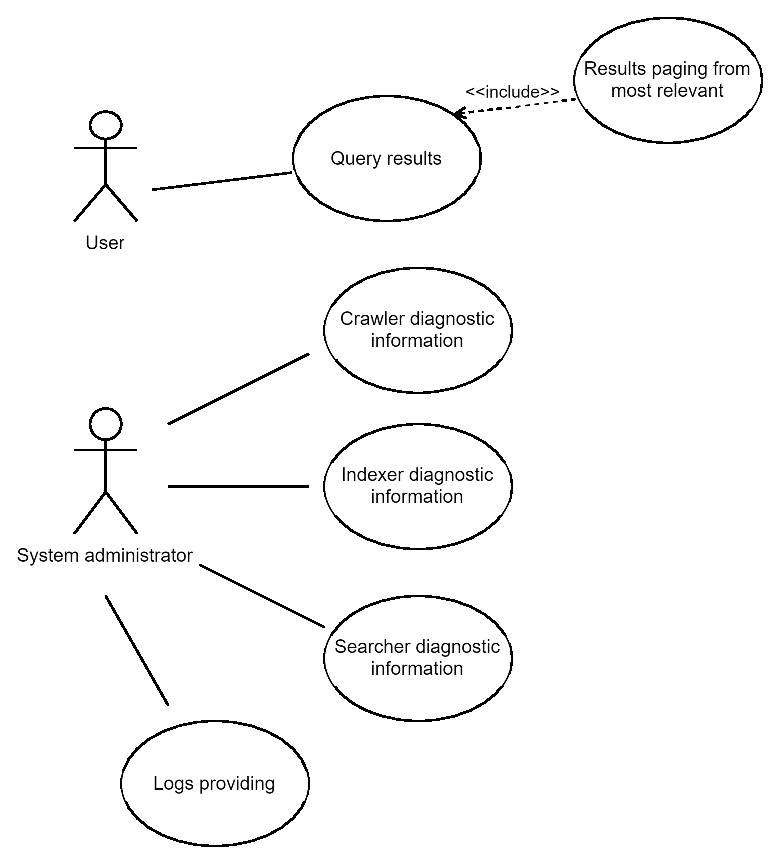
\includegraphics[width=1\linewidth]{diagram_usecases}}
\caption{Диаграмма вариантов использования системы}
\label{diagram_usecases:image}
\end{figure}

Диаграмма развертывания программно-информационной системы показана на рисунке 2.4.

\begin{figure}
\center{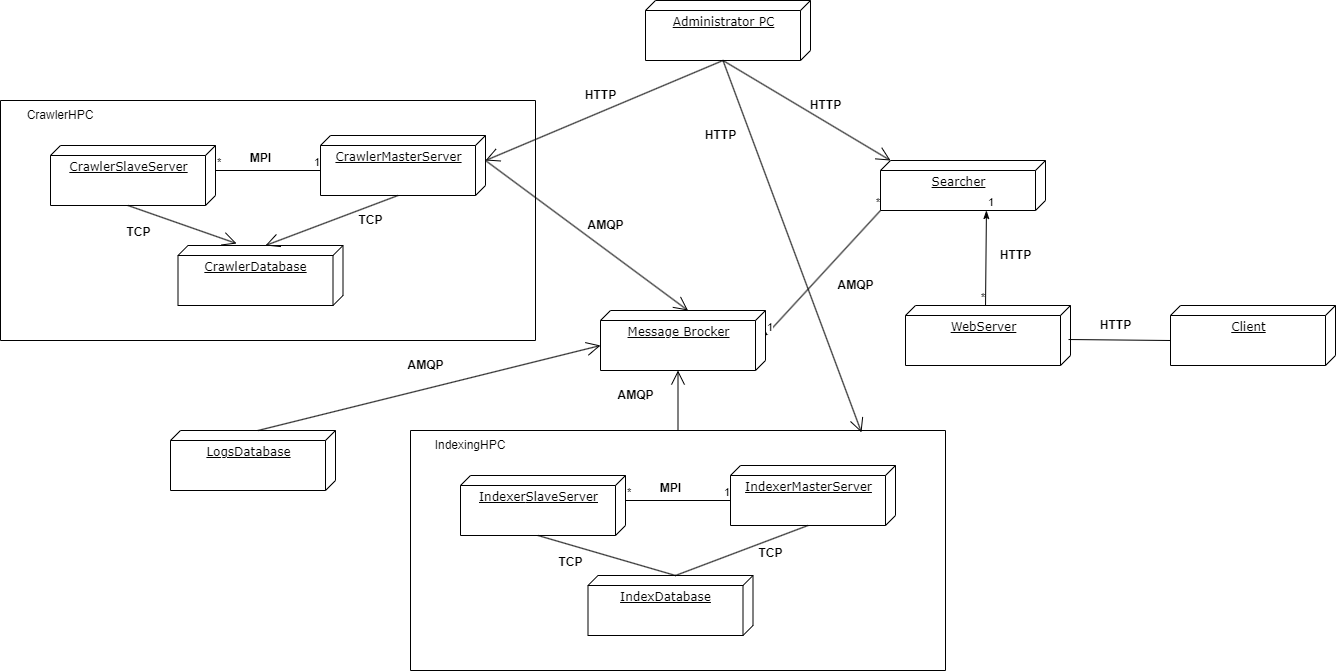
\includegraphics[width=1\linewidth]{diagram_deployment}}
\caption{Диаграмма развертывания системы}
\label{diagram_deployment:image}
\end{figure}

\subsubsection{Требования пользователя к интерфейсу web-сайта}

Сайт должен включать в себя:
\begin{itemize}
	\item стартовую страницу поиска с полем для ввода запросов;
	\item страницу с отображенными результатами поиска;
	\item механизм парцеального отображения результатов с возможностью страничной навигации.
\end{itemize}

На рисунках 2.1 - 2.2 представлены макеты веб-сайтов для взаимодействия пользователя с системой.
\begin{figure}
\center{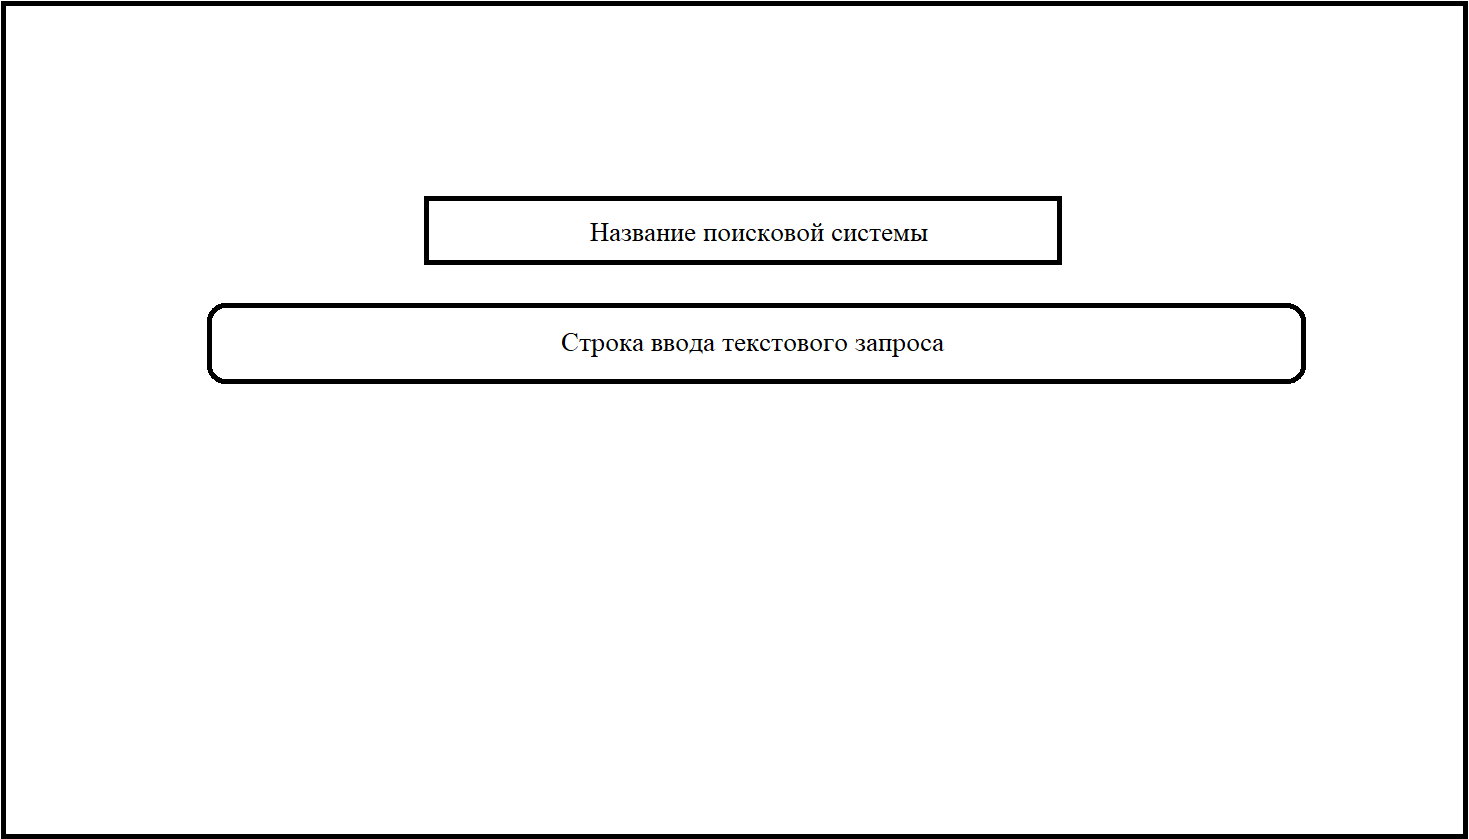
\includegraphics[width=1\linewidth]{site_main}}
\caption{Главная страница поискового веб-сайта}
\label{site_main:image}
\end{figure}
\begin{figure}
\center{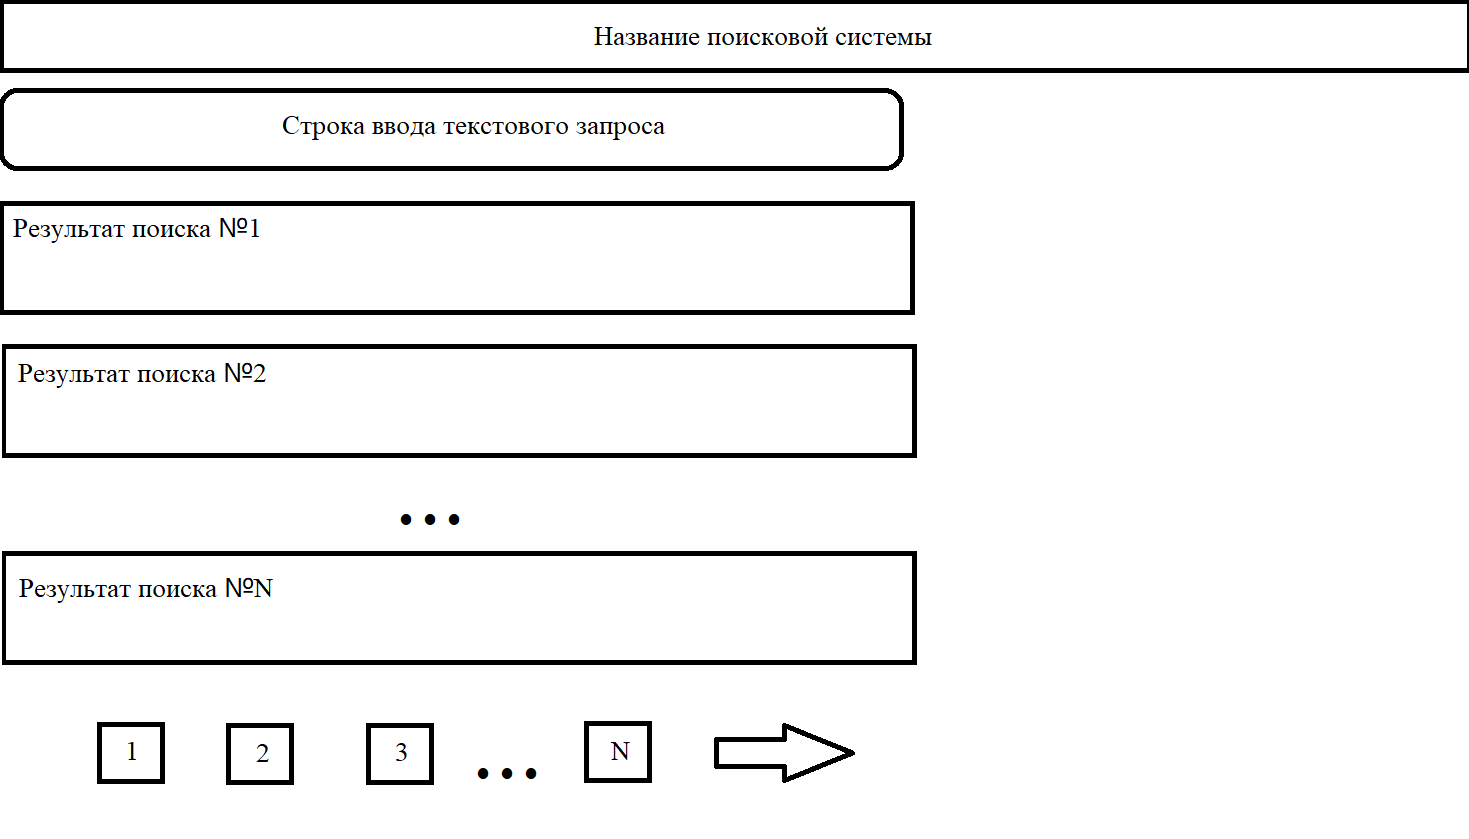
\includegraphics[width=1\linewidth]{site_search}}
\caption{Страница отображения результатов поиска}
\label{site_search:image}
\end{figure}


\subsection{Требования к оформлению документации}

Разработка программной документации и программного изделия должна производиться согласно ГОСТ 19.102-77 и ГОСТ 34.601-90. Единая система программной документации.
